\chapter{Prediction and analysis of gene function}
\label{chap:intro}
%%%%%%%%%%%%%%%%%%%%%%
%%%%%%%%%%%%%%%%%%%%%%
%\section{Introduction}
%%%%%%%%%%%%%%%%%%%%%%
%%%%%%%%%%%%%%%%%%%%%%


	Characterizing the functional behavior of individual proteins in a variety of different contexts is an important step in understanding life at the molecular level.  Endeavors such as understanding biological pathways, investigating disease, and developing drugs to cure those diseases depend on being able to describe the actions of individual proteins, both in terms of their physiochemical molecular function, involvement in biological processes, and the sub-cellular location at which these actions are carried out.
		%\textcolor{red}{give some example of how this individualized approach has made progress.  find a disease.  maybe speak about lacz}
In spite of the fact that there are increasingly more tools for the interrogation of protein behavior, there are still a large number of functionally uncharacterized proteins, with the gap between known sequences and experimentally characterized ones growing at an exponential pace (\Cref{fig:growth}). Currently, there are about $50,000$ proteins with at least one experimentally annotated Gene Ontology (GO) term in Swiss-Prot \citep{bairoch2005universal}. However, owing to the numerous sequencing projects \citep{Liolios2008}, the gap between annotated and non-annotated proteins has exceeded two orders of magnitude, and will only become wider. There is also a large amount of disparity in the distribution of experimental annotations among organisms, with most annotations occurring in model organisms  (\Cref{fig:per_organism}).  Furthermore, while most experimentally annotated proteins come from model organisms, with the exception of yeast, less than half of the genome of any model organism has yet to be assigned experimentally characterized GO functions. The numbers in \Cref{fig:per_organism} do not illustrate the fact that many annotations are quite vague. Because of  the multitude of ways a protein's function can be characterized, having a single annotation does not mean that protein has been fully annotated.   For example, $26\%$ of proteins with experimentally characterized molecular function annotations in the January 2011 version of Swiss-Prot have �protein binding� as their most specific molecular function term.


%%%%%%%%%%%%%%%%%%%%%%
%%%%%%%%%%%%%%%%%%%%%%
\begin{figure*}[h!]
\begin{centering}
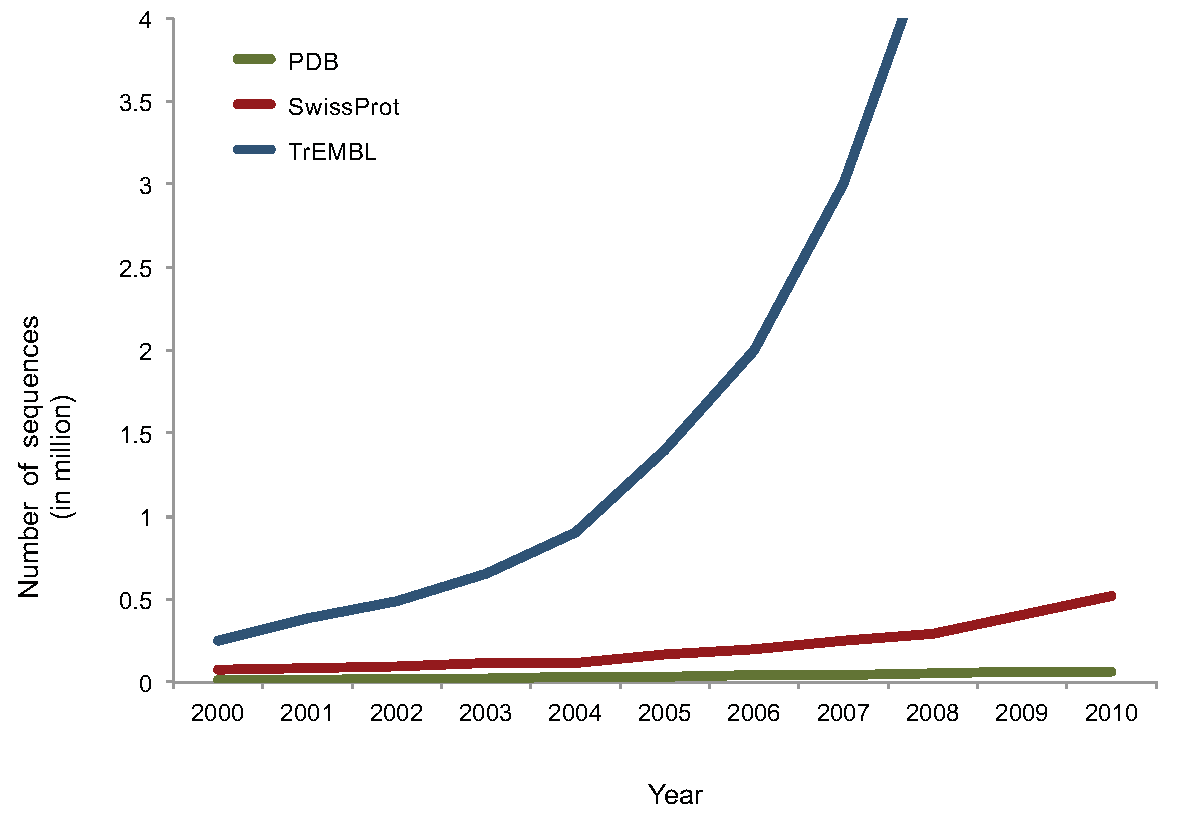
\includegraphics[width=0.70\linewidth]{Figures/intro/Fig_1B}
\end{centering}
\caption[Growth of databases]{The growth in the number of entries in three major databases is shown in millions of sequences. TrEMBL represents the compendium of all known sequences, regardless of how well characterized they are. PDB represents all sequences for which a structure has been experimentally determined. Swiss-Prot is a database of confirmed and relatively well characterized proteins, although not all proteins have been assigned experimentally verified GO annotations.}
\label{fig:growth}
\end{figure*}
%%%%%%%%%%%%%%%%%%%%%%
%%%%%%%%%%%%%%%%%%%%%%




%%%%%%%%%%%%%%%%%%%%%%
%%%%%%%%%%%%%%%%%%%%%%
\begin{figure*}[h!]
\begin{centering}
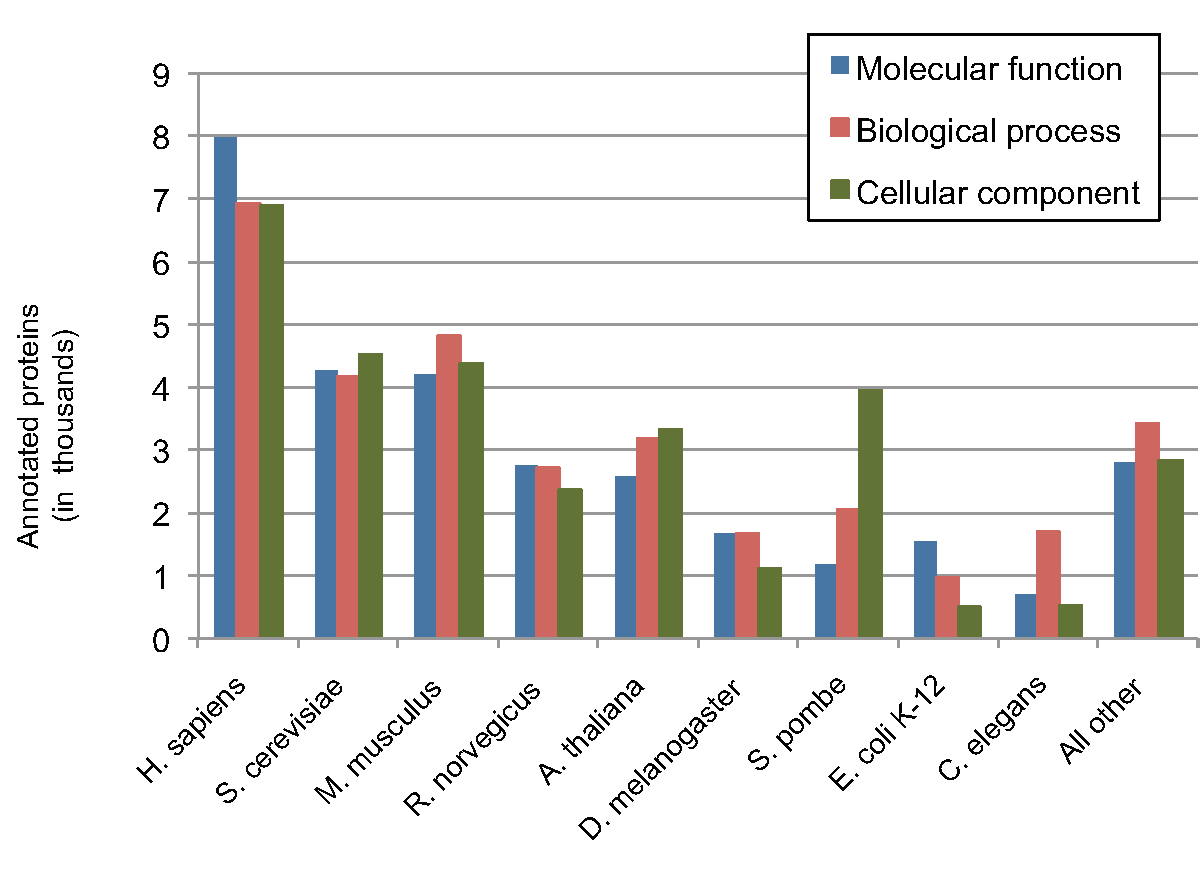
\includegraphics[width=0.70\linewidth]{Figures/intro/Fig_1A}
\end{centering}
\caption[Distribution of sequences with experimental annotations amongst model organisms]{The distribution of experimentally annotated (EXP, TAS and IC evidence codes) proteins amongst well characterized organisms and all other organisms for the three branches of the Gene Ontology. Annotations were taken from the January 2012 version of Swiss-Prot.}
\label{fig:per_organism}
\end{figure*}
%%%%%%%%%%%%%%%%%%%%%%
%%%%%%%%%%%%%%%%%%%%%%


Because of the growing disparity between known and experimentally annotated proteins, and the financial and ethical restrictions placed on experimentally interrogating function, \emph{in silico} methods hold the greatest promise in making progress towards functionally characterizing the large compendium of known proteins.  This dissertation is largely focused on \emph{in silico} efforts to infer protein function. Because our ability to draw reliable conclusions about the performance of one technique over another is grounded in having reliable benchmarking methods a great deal of attention is also paid to this topic (\Cref{ch:rumi}).


\section{Defining function}

%Because the central unifying theme to this dissertation if protein function, it is perhaps important to take some time to define what it means when we talk about ``function".  In natural parlance the term function would be taken to mean the purpose, or reason for something.  The function of a chair is to serve as a place for someone to sit; the function of a pencil is to write.  Several approaches to defining function in biological context have been taken to account for the strong undertones of intentionality in the everyday definition of function.  Evolution is by all means a blind process. Two contrasting definitions of function are the selected effect and causal role definitions.  
%
%The selected effect definition of function \citep{millikan1989defense} defines the function of a biological entity, be it an organ, appendage, or gene; as the role or effect for which the entity was \emph{selected}. Obviously, again, the definition of the term \emph{select} differs from our every day use.  A particular gene obviously is not selected in the same way I select a shirt to start the  For example, a particular gene does not increase in frequency, and possibly go to fixation, under certain conditions because some force is selecting it any more than carbon forms diamonds under certain conditions because that structure of atoms is being \emph{selected},.  

%Although we would easily contend that there are \emph{forces}, like gravity or weather, at work in the world there is no intentionality at work , as implied by the use of the term selection, merely causes (past) and consequences (future). As a consequence of high levels of pressure and long amounts of time carbon atoms are rearranged into a symmetric lattice forming diamonds. Similarily, as a consequence of high level of arsenic in some environments genes associated with processing arsenic rise in frequency. When one neutralizes the term selection the selected effect definition of function can seem odd.  Is it the function of diamonds to p[rocess high pressure?  

%In contrast, the causal role definition simply defines the function of an entity as the role it carries out.  
%It does not design a chair by first asking for a place to sit; nor does it design a chair, the chair simply arises randomly.
%
%This dissertation addresses protein function at the molecular function and biological process levels, as defined by the GO consortium. 
%
%
%Give a brief overview of the various definitions of function.  Focus on the selected effect and causal role definitions of function.  
%
%Categorize the use of function in the context of the gene ontology.
%
%Distance yourself from any teleological explanations.  

In light of the fact that the central unifying theme to this dissertation is protein function, it is perhaps important to take some time to define what it means when we talk about ``function". This dissertation addresses protein function, as defined by the GO consortium \citep{Ashburner2000}. Although alternative definitions exist \citep{millikan1989defense}, in practice function is generally considered from the causal role perspective \citep{amundson1994function}. In a very broad sense protein function is a multi-scale concept that reflects ``everything that happens to or through a protein" \citep{Rost2003}, and is typically considered from the biochemical, biological, and phenotypic perspectives \citep{Bartlett2003}. How the function of a protein is defined is largely dependent on the perspective from which it is being studied. From the biochemical, or molecular, perspective a protein may be a kinase, whereas in terms of its biological function this kinase can be involved in numerous processes, such as cell cycle regulation or cell-cell signaling. Two proteins with the same molecular function may be involved in drastically different biological processes, and conversely, the set of proteins associated with a particular biological process will generally be drawn from a wide range of molecular functions. From the phenotypic viewpoint, a protein is generally associated with variation in observable physical or behavioral traits. For example, kinase variants or mutants may be responsible for disease. Adding another level of complexity to the study of function is the fact that a protein's molecular function, while generally considered to be a static notion, is modulated by a particular cellular context, e.g. the presence of other molecules, or properties of the physical environment, e.g. temperature \citep{Mohan2009}.

Several classification systems have been proposed to standardize functional annotation and to facilitate computation. With few exceptions, these classification systems usually take on the structure of hierarchical ontologies. Enzyme Commission (EC) numbers \citep{NC_IUBMB_1992} and the MIPS functional catalogue \citep{Ruepp2004} are two well-accepted schemes; however, the most commonly used functional classification is the Gene Ontology (GO). GO provides three hierarchical classifications as directed acyclic graphs: molecular function ontology, biological process ontology, and cellular component \citep{Ashburner2000}. With respect to defining a particular gene's phenotype, the  Human Phenotype Ontology \citep{Robinson2010}, Unified Medical Language System \citep{Bodenreider2004} and Disease Ontology \citep{schriml2012disease} are human specific and predominantly constructed to address human disease. In the case of the Unified Medical Language System the focus in on defining associations between genes and medical disorders.
Several ontologies provide organism independent terminology for defining phenotype such as the Vertebrate Skeletal Anatomy Ontology \citep{dahdul2012unified}.  

 %It is unclear whether the working definition of function used by GO conforms to the selected effect definition of function \citep{millikan1989defense}, but this is more a consequence of the evidence codes allowed than the actual terms in the ontology.


\section{Challenges in predicting function}
\label{sec:challenges}

%%%%%%%%%%%%%%%%%%%%%%
%%%%%%%%%%%%%%%%%%%%%%
\subsection{Multi-functional proteins}
%%%%%%%%%%%%%%%%%%%%%%
%%%%%%%%%%%%%%%%%%%%%%

In order to properly design a predictor of function it is important to consider how the classification task should be framed. It is well-known that some proteins have the ability to carry out more than one function, or ``moonlight" \citep{Jeffery1999,Jeffery2009}. Such abilities can be facilitated by either having multiple functional domains, a single domain which binds multiple partners, or by different behavior upon post-translational modifications or change in physiological conditions \citep{Jeffery2004,Jeffery2009}. Furthermore, there are also multiple terms that could be associated with what could be considered a single function.  For example, a protein could be involved in RNA transcription, but be annotated with both ``nucleic acid binding" and ``RNA polymerase."   

We systematically analyze multi-functionality with respect to molecular function and biological process terms in GO. As an approximation of distinct functions we only consider the number of experimentally determined leaf GO terms associated with each protein. A GO term $g$ was included in the count if no other term associated with the protein had $g$ as its more general term in the ontology. For example, if a protein is associated with the term ``protein binding", the term ``binding" is not counted as distinct function because it is a generalization of ``protein binding"; however, the term ``nucleic acid binding" would be counted because neither of the two terms is a generalization of the other.

\Cref{fig:fanngo1} shows the distribution of the number of leaf terms associated with each functionally annotated sequence for both ontologies. In total, $26,707$ sequences were included in the molecular function analysis and $29,118$ sequences were included in the biological process analysis. Only experimental evidence, traceable author's statement, or curator's inference were taken from Swiss-Prot v15.15 (exclusion of traceable author's statement and curator's inference resulted in very similar distributions; data not shown). The plots show greater diversity in a protein's participation in a biological process than its ability to carry out distinct molecular functions. About $66\%$ of the proteins experimentally annotated by molecular function terms have only $1$ leaf term, with no protein having more than $14$. On the other hand, only $44\%$ of proteins have only $1$ biological process leaf term, with $6$ proteins having $50$ terms or more. This is consistent with the expectation that biological processes are governed more by the context in which a protein is utilized, and less by the physicochemical abilities of the protein. Interestingly, both the molecular function and biological process ontologies show a negative exponential decrease in the probability that a protein is associated with an increasing number of functional terms. 

Given the incompleteness of experimental annotations and the propensity of researchers to focus on individual genes it is expected that the number of multi-functional proteins will only increase. In the context of protein function prediction, these distributions suggest there is a level of sophistication that should be required from a computational method with respect to its outputs.  Function prediction should clearly not be approached as a binary, or even a multi-class classification problem; but as a multi-label classification, or structured learning problem where it should be expected that data points will be more than one out of many labels.

%%%%%%%%%%%%%%%%%%%%%%
%%%%%%%%%%%%%%%%%%%%%%
\begin{figure*}[h!]
\begin{centering}

\includegraphics[width=\linewidth]{Figures/fanngo/Figure_1}
\par\end{centering}
\caption[The distribution of leaf terms counts per ontology]{The distribution of the number of leaf terms in (A) Molecular Function and (B) Biological Process ontologies. The x-axis represents the number of leaf terms associated with a protein; the y-axis represents the fraction of proteins in the data set with the given number of leaf terms. Both axes are in $\log_{10}$ scale. The inset in each panel provides a pie chart that corresponds to each plot.}
\label{fig:fanngo1}
\end{figure*}
%%%%%%%%%%%%%%%%%%%%%%
%%%%%%%%%%%%%%%%%%%%%%

We also analyzed the relationship between the number of molecular functions and biological processes a protein is associated with. It seems intuitive to postulate that proteins with the ability to carry out multiple molecular functions should be more easily utilized in multiple different contexts, giving rise to an association with more biological processes. Out of $19,240$ proteins in the intersection of data sets for molecular function and biological process, we found a Pearson correlation coefficient of $0.261$ between the numbers of associated leaf terms in the two ontologies. While this correlation may seem weak, we determined that this value is statistically significant by using a permutation test where the numbers of molecular function and biological process terms were permuted in the data set of proteins. We carried out $100,000$ such permutations and did not find any cases in which the correlation coefficient was $0.261$ or greater (the mean correlation coefficient for permuted data was $6.1\times10^{-6}$ and standard deviation was $7.2\times 10^{-3}$). 

While, in general, a protein performing multiple molecular functions is associated with multiple biological processes, we conducted further analysis of proteins associated with a single term from one ontology and multiple terms from the other. For example, among the proteins that have only one molecular function leaf term, but multiple biological process terms, we found that receptor binding terms such as ``chemokine receptor binding" and ``cytokine receptor binding" are the most enriched ($P < 1.0\times10^{-7}$; Binomial test). On the other hand, there are also cases in which proteins that are associated with only one leaf term in biological process are related to multiple molecular function terms. Such biological process terms are almost all related to metabolic processes, e.g. ``cellular metabolic process", ``primary metabolic process", etc. ($P < 1.0\times10^{-7}$; Binomial test). When analyzing this class of proteins we also found that some terms did not occur as often as expected.  When looking at the class of proteins with one molecular function term and multiple biological process terms we found that ``catalytic activity" was depleted. While sequences are annotated with this term $28\%$ of the time in the whole data set ($29\%$ in the set of all proteins with single molecular function leaf term), it only occurs $17\%$ of the time when we only consider sequences with exactly one molecular function term but $3$ or more biological process terms associated with them. Similarly, proteins having $1$ biological process leaf term, but few molecular function terms are usually involved in reproduction. We note that this data needs to be interpreted with caution, because molecular function and biological process terms are incomplete for most proteins and also because there may exist biases in ways current functions are acquired.

%Finally, we looked at the relationship between the number of Pfam domains \citep{Finn2008} found in a protein and the number of biological process and molecular function terms it was associated with. We found that the Pearson correlation between the number of molecular function leaf terms and Pfam domains (detected using a threshold of $0.001$) was much larger than that of biological process leaf terms and Pfam domains ($0.126$ and $0.090$ respectively). While, again, these correlation values might seem small, we found both were significant using the permutation test.



%%%%%%%%%%%%%%%%%%%%%%
%%%%%%%%%%%%%%%%%%%%%%
\subsection{Transfer of function by sequence similarity}
%%%%%%%%%%%%%%%%%%%%%%
%%%%%%%%%%%%%%%%%%%%%%

Because transferring function based on sequence similarity is one of the most intuitive, and easy to implement methods for inferring function it is important to consider its effectiveness. We evaluated the performance of simple function transfer between similar sequences. The following steps were taken: for each range of pairwise global sequence identities, a target protein received all functional terms from each experimentally annotated protein within the given sequence identity range (regardless of the species). For each target sequence with more than one match in the given identity range the precision and recall (see \Cref{sec:fanngomodels}) were calculated as averages over all pairs. Then, the precision and recall for the entire data set are reported (\Cref{fig:fanngo2}) as averages of the averaged precisions and recalls calculated for each sequence covered (a leave-one-out estimation). We also report the coverage for each range of sequence identity as the fraction of proteins with at least one other annotated sequence whose pairwise sequence identity falls within the defined range. Finally, for all covered sequences we report the percentage of perfect annotations, i.e. the percentage of all pairwise annotations in a given bin where both precision and recall were 1.

%%%%%%%%%%%%%%%%%%%%%%
%%%%%%%%%%%%%%%%%%%%%%
\begin{figure*}[h!]
\begin{centering}
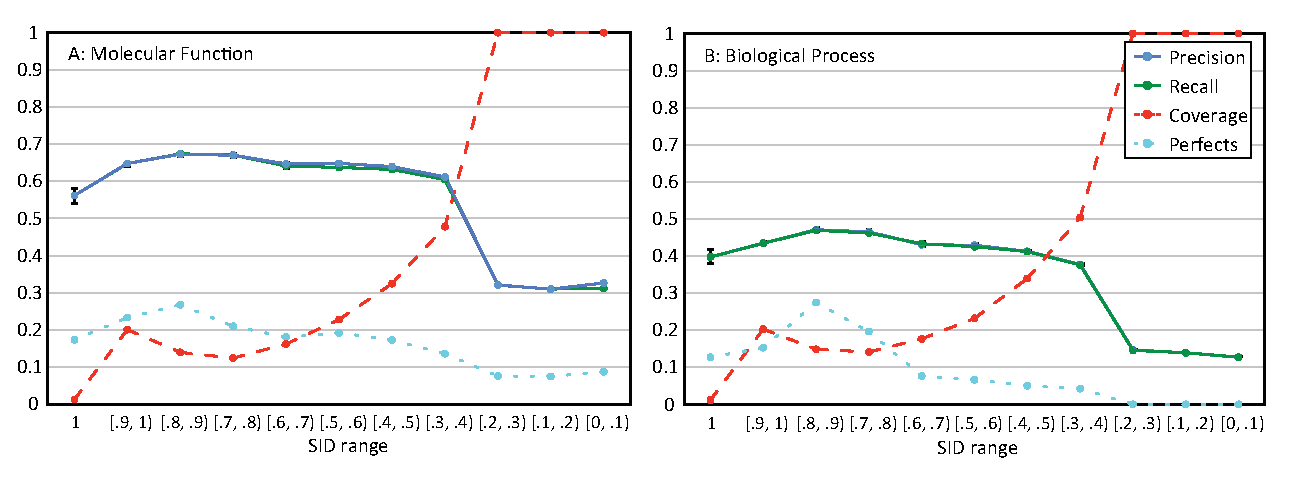
\includegraphics[width=\linewidth]{Figures/fanngo/Figure_2}
\par\end{centering}
\caption[Accuracy of function transfer using global sequence identity]{Accuracy of function transfer using global pairwise sequence identities (A: Molecular Function; B: Biological Process). For each sequence identity range (x-axis), shown are the average precision (blue solid line) and recall (green solid line) of function transfer by pairwise similarity. The teal dotted line represents the percentage of pairs with perfect annotations (e.g. both precision and recall equal to 1). The red dashed curve represents the percent of proteins that have pairwise matches (annotated with GO terms; experimental evidence code) in a given range. The error bars represent 95\% confidence intervals.}
\label{fig:fanngo2}
\end{figure*}
%%%%%%%%%%%%%%%%%%%%%%
%%%%%%%%%%%%%%%%%%%%%%

The results shown in \Cref{fig:fanngo2} suggest that using global sequence identity for the transfer of functional annotations is only moderately accurate (pairwise local alignments performed similarly; data not shown). Surprisingly, even for $100\%$ identity transfer of function does not achieve either precision or recall of $1$ (only $17\%$ of identical sequence pairs had perfect transfer of molecular function and $12\%$ of biological process terms). This relatively low rate of perfect annotations among perfect matches, and similarly in the remaining identity bins, in our data set is caused by three factors: (i) sparsity of database annotations, where proteins are incompletely annotated with respect to functionality and also specificity of annotation; (ii) database errors, caused by incorrect interpretation of experiments or by curation errors, \citep{Brenner1999,Schnoes2009} and (iii) organismal context, where the difference between two organisms influences a particular functional role of individual proteins, even at $100\%$ sequence identity.

In general, transferring molecular function annotations is more accurate than transferring biological process annotations, which has previously also been observed by Rogers and Ben-Hur in a different prediction scenario \citep{Rogers2009}. This is probably a result of the fact that molecular function terms are less dependent upon cellular, tissue, or organismal context, but also that the topological properties, including the average branching factor, the number of terms, and the average depth of a leaf node, between the two ontologies differ (data not shown). For both ontologies the precision of transferring predictions rapidly decreases once the $20-30\%$ identity is reached. This range of sequence identity has been termed the ``twilight zone" for the inference of protein structure from sequence \citep{Rost1999}. In the context of function transfer such a twilight zone cannot be clearly defined (or rather should be extended to the entire range $30-100\%$), with the range below $30\%$ being one where function transfer breaks down completely (``midnight zone"). We also evaluated an alternative approach where functional terms from all matches in a given identity range were transferred to the target protein and found a very similar level of precision but an increased recall (\Cref{fig:fanngoS1}).

%%%%%%%%%%%%%%%%%%%%%%
%%%%%%%%%%%%%%%%%%%%%%
\begin{figure*}[h!]
\begin{centering}
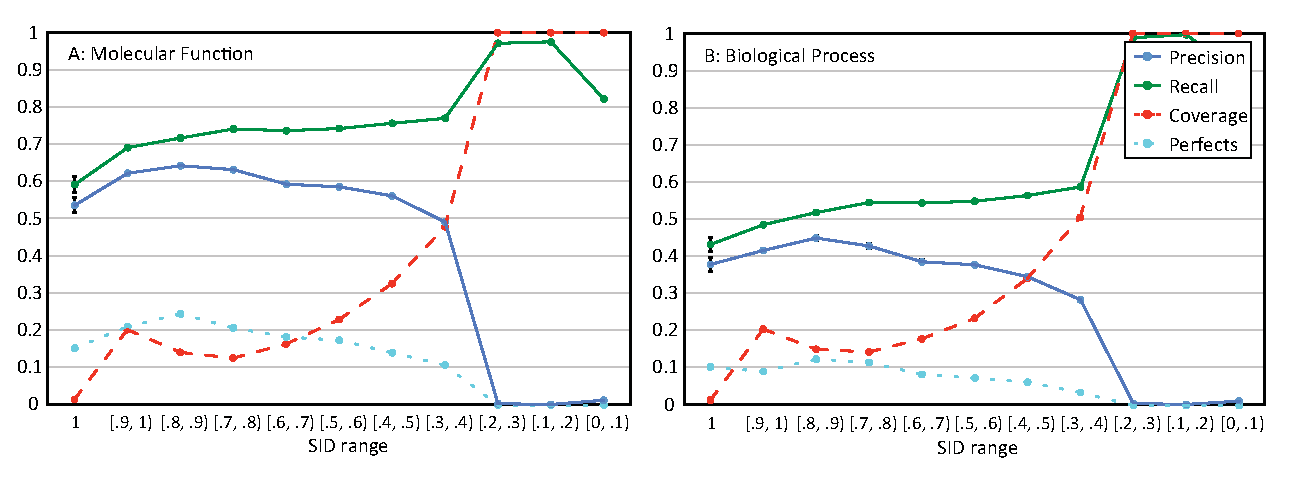
\includegraphics[width=\linewidth]{Figures/fanngo/Supplementary_Figure_1}
\par\end{centering}
\caption[The precision and recall of function transfer using global pairwise sequence identities]{The precision and recall of function transfer using global pairwise sequence identities (A: Molecular Function; B: Biological Process). For each sequence identity range (x-axis), shown the average precision (blue solid line) and recall (green solid line) of function transfer were calculated by annotating a target sequence with the annotations of all hits within a particular SID range. The precision and recall curves in this figure differ from those in Figure 2 in that precision and recall for an individual data-point here do not represent an average for each hit, but instead the agglomeration of all terms from hits for a particular range of SID.  The teal dotted line represents the percentage of pairs with perfect annotations (e.g. both precision and recall equal to 1). The red dashed curve represents the percent of proteins that have pairwise matches (annotated with GO terms; experimental evidence code) in a given range. The error bars represent 95\% confidence intervals.}
\label{fig:fanngoS1}
\end{figure*}
%%%%%%%%%%%%%%%%%%%%%%
%%%%%%%%%%%%%%%%%%%%%%

The quality of function transfer is highly dependent on the particular class of protein. We show this by splitting the molecular function/biological process data sets into enzymes (proteins annotated with term ``catalytic activity"), and non-enzymes. As seen in \Cref{fig:fanngo3}, the ability to transfer molecular functions to these two classes of proteins was noticeably different and most likely points to a higher quality of functional annotations for enzymes.

%%%%%%%%%%%%%%%%%%%%%%
%%%%%%%%%%%%%%%%%%%%%%
\begin{figure*}[h!]
\begin{centering}
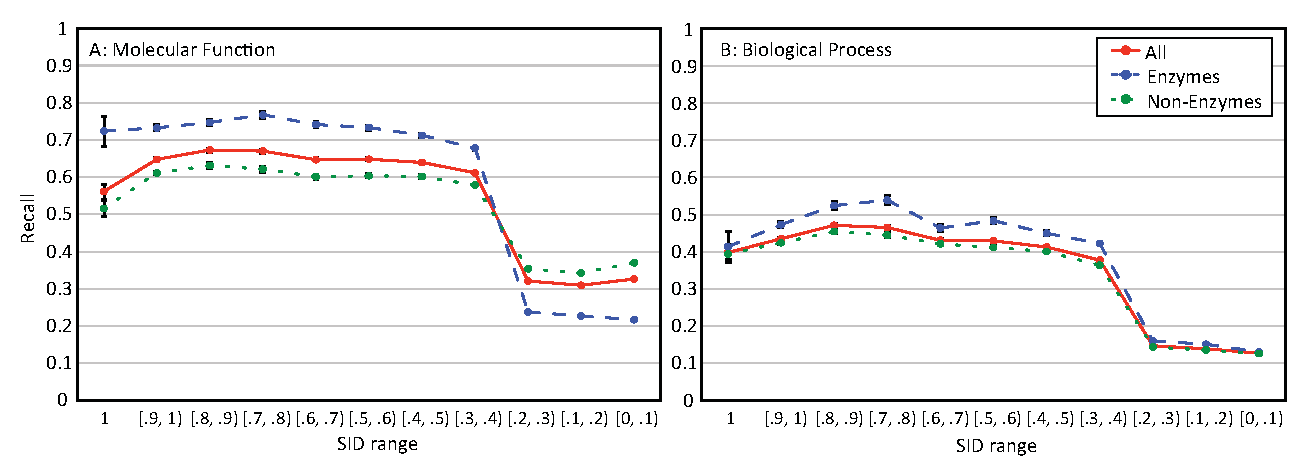
\includegraphics[width=\linewidth]{Figures/fanngo/Figure_3}
\par\end{centering}
\caption[Accuracy of function transfer using global pairwise sequence identities for enzymes vs. non-enzymes]{Accuracy of function transfer using global pairwise sequence identities for enzymes vs. non-enzymes (A: Molecular Function; B: Biological Process). For each sequence identity range (x-axis), shown is the average precision of function transfer by pairwise similarity (blue dashed line: enzymes, green dotted line: non-enzymes; red solid line: combined). The error bars represent 95\% confidence intervals}
\label{fig:fanngo3}
\end{figure*}
%%%%%%%%%%%%%%%%%%%%%%
%%%%%%%%%%%%%%%%%%%%%%

Another interesting trend in the data is the fact that the quality of annotations transferred between sequences from the same species is higher than that obtained between different species. This can be seen by comparing the precision/recall curves in \Cref{fig:fanngo4} obtained by only considering pairs of sequences from the same species (``within" curve, blue line), and only considering pairs of sequences from different organisms (``between" curve, green line). A similar trend has been previously observed on protein-protein interaction data by \citep{Mika2006}.

%%%%%%%%%%%%%%%%%%%%%%
%%%%%%%%%%%%%%%%%%%%%%
\begin{figure*}[h!]
\begin{centering}
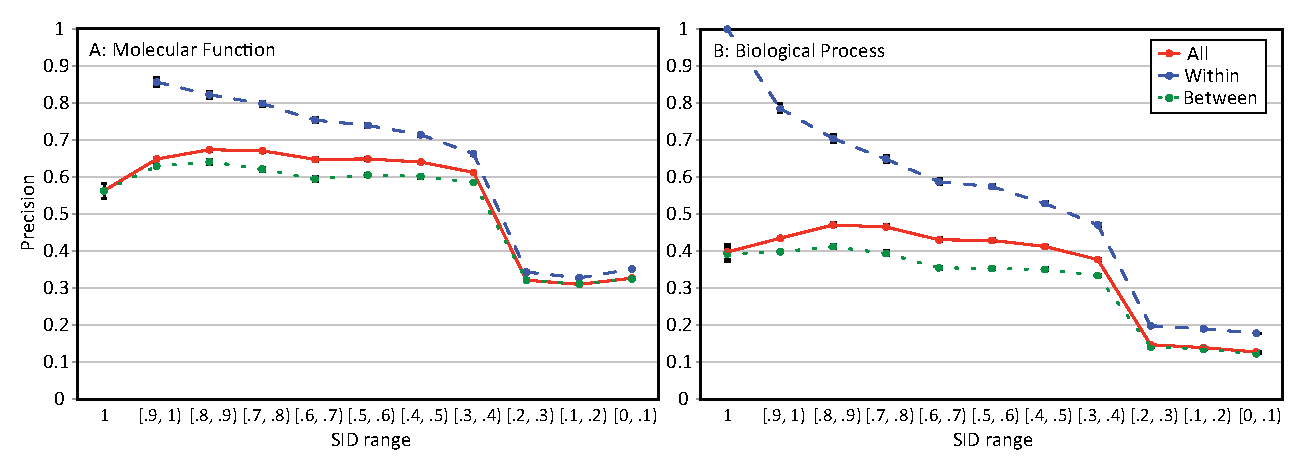
\includegraphics[width=\linewidth]{Figures/fanngo/Figure_4}
\par\end{centering}
\caption[Accuracy of function transfer using global pairwise sequence identities from the same or different organism]{Accuracy of function transfer using global pairwise sequence identities from the same or different organism (A: Molecular Function; B: Biological Process). For each sequence identity range (x-axis), shown is the average precision of function transfer by pairwise similarity (blue dashed line: same organism, green dotted line: different organism; red solid line: combined). The error bars represent 95\% confidence intervals.}
\label{fig:fanngo4}
\end{figure*}
%%%%%%%%%%%%%%%%%%%%%%
%%%%%%%%%%%%%%%%%%%%%%

The disappointing performance of transferring function based on sequence similarity highlights the importance of developing advanced methods for inferring function.  Although many data bases provide electronic annotations for proteins, we are not aware the quality of these methods had not been assessed until our publication \citep{Clark2011}. Below we consider the quality electronic annotations in Swiss-Prot.

%%%%%%%%%%%%%%%%%%%%%%
%%%%%%%%%%%%%%%%%%%%%%
\subsection{Quality of non-experimental annotations in Swiss-Prot}
%%%%%%%%%%%%%%%%%%%%%%
%%%%%%%%%%%%%%%%%%%%%%

Protein databases such as GO or Swiss-Prot contain a number of functional annotations supported by non-experimental evidence codes. Because of the ability of these annotations to preclude prediction efforts it is important to consider their quality.  We aimed to assess the quality of such annotations by analyzing non-experimental annotations for the proteins in Swiss-Prot (v10.0-v15.0) that in a later release (v15.15) accumulated experimental annotations.  \Cref{fig:fanngo5} shows the quality of annotations by non-traceable author statement (NAS) or inferred from electronic annotation (IEA) evidence codes (the remaining non-experimental codes did not contain enough sequences). Using the current annotations (v15.15) as true function, the precision and recall of each protein's annotation were calculated (\Cref{fig:fanngo5}). 

%%%%%%%%%%%%%%%%%%%%%%
%%%%%%%%%%%%%%%%%%%%%%
\begin{figure*}[h!]
\begin{centering}
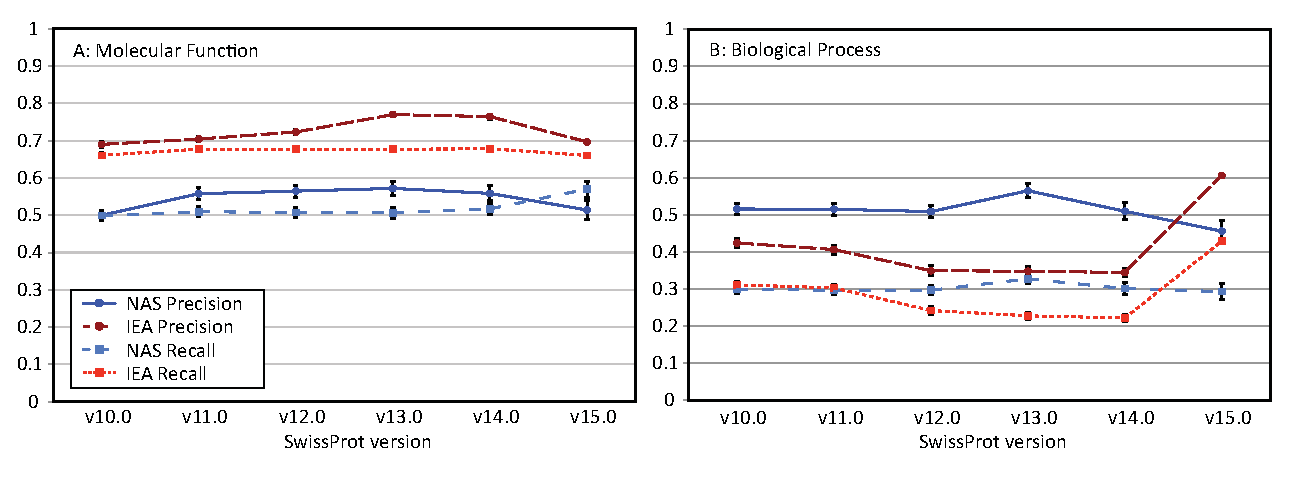
\includegraphics[width=\linewidth]{Figures/fanngo/Figure_5}
\par\end{centering}
\caption[Accuracy of function transfer between different versions of the Swiss-Prot database]{Accuracy of function transfer for the Swiss-Prot database (A: Molecular Function; B: Biological Process). X-axis represents a different version of Swiss-Prot. The dark dashed red line represents the precision of IEA annotations and the dark blue solid line represents the precision of NAS annotations. The light red dotted line represents the recall of IEA annotations, and the light blue dashed line represents the recall of NAS annotations. The error bars represent 95\% confidence intervals.}
\label{fig:fanngo5}
\end{figure*}
%%%%%%%%%%%%%%%%%%%%%%
%%%%%%%%%%%%%%%%%%%%%%

As shown in \Cref{fig:fanngo5}, the quality of electronic annotations is consistently better than that of non-traceable author statements for molecular function, while the trend is reversed for biological process. Interestingly, the precision of the electronic annotations in the Swiss-Prot database for molecular function exceeds the level achieved  (\Cref{fig:fanngo2}), while the NAS evidence suggest lower confidence levels compared to that of sequence transfer. A historical analysis of biological process annotations suggests that neither electronic annotation, nor non-traceable author statements, have been at the level of simple transfer of annotation; however the latest major release of Swiss-Prot (v15.0) provides more accurate electronic inference than transfer by sequence similarity. Similar results were found by a later paper \citep{vskunca2012quality}, which serves to reinforce our initial findings that there is room for improvement in deposited electronic annotations. 

%%%%%%%%%%%%%%%%%%%%%%
%%%%%%%%%%%%%%%%%%%%%%
\section{State of the art methods}
%%%%%%%%%%%%%%%%%%%%%%
%%%%%%%%%%%%%%%%%%%%%%

Historically, sequence-based inference was the first strategy used to predict protein function, even if most studies at the time avoided explicitly relating homology and function \citep{Doolittle1986}. Global and local sequence alignments were used to query sequence databases for similarities with a target protein. With the accumulation of experimentally determined protein functions, the most similar annotated sequences have traditionally been used to infer function \citep{Rost2003}.  Several methods have developed novel techniques for utilizing sequence alignment information as input to supervised learning methods \citep{Clark2011,Wass2008,kourmpetis2013gene,minneci2013ffpred,Sokolov2010}. More advanced methods exploited predicted physicochemical properties \citep{Jensen2002,Jensen2003,minneci2013ffpred,cozzetto2013contribution}, evolutionary relationships \citep{enault2005phydbac,Engelhardt2005,gaudet2011phylogenetic,marcotte1999detecting,Pellegrini1999,Bandyopadhyay2006b}, or the structure of functional ontologies in order to achieve different confidence levels for different ontological terms \citep{Barutcuoglu2006,Hawkins2006,Martin2004}. Microarrays \citep{huttenhower2006scalable}, protein-protein interaction networks \citep{Deng2003,Letovsky2003,Vazquez2003,Nabieva2005}, protein structures \citep{Laskowski2008,Pazos2004,Pal2005,Hermann2007} or a combination of data types \citep{costello2009gene,kourmpetis2010bayesian,Lee2004,Troyanskaya2003,Sokolov2010} have also been exploited. However, most of these methods are limited to a few organisms where such data are available.  One way or another, sequence alignment-based inference is the cornerstone of functional inference \citep{Radivojac2013,hamp2013homology}.

Sequence alignment-based transfer of function has been thoroughly studied in the last decade, predominantly for enzymes \citep{Addou2009,Devos2000,Rost2003,Tian2003,Todd2001,Wilson2000}. The results of these studies indicate that at least $60\%$ sequence identity, and more likely closer to $80\%$, is required for the accurate transfer of the third level of EC classification. More sophisticated approaches were proposed as well: the GOtcha method was developed in order to take sequence alignment scores between a query protein and a functionally annotated database and overlay them on the functional ontology, cumulatively propagating such scores \citep{Martin2004}. PFP refined this technique by incorporating PSI-BLAST alignments at very low significance levels and conditional probabilities that a protein is associated with pairs of functional terms \citep{Hawkins2006}. Other methods such as ProtFun \citep{Jensen2003}, ConFunc \citep{Wass2008}, GOsling \citep{Jones2008a}, and GOstruct \citep{Sokolov2010} were developed for high-throughput prediction tasks. Finally, phylogenetic methods attempt to exploit particular evolutionary relationships within a gene family \citep{Brown2006,Eisen1998}. Methods such as SIFTER \citep{Engelhardt2005} or ortholog identification methods \citep{Remm2001} belong in this category. Several recent reviews provide good perspectives on protein function prediction at all scales \citep{Dalkilic2008,Friedberg2006,Kann2007,Laskowski2008,Lee2007,Punta2008,Rentzsch2009,Rost2003}.

\subsection{Community-wide assessment of function prediction}

%\begin{figure*}[t!]
\begin{centering}
	\begin{subfigure}[b]{0.85\textwidth}
                \centering
		\caption{Timeline}
                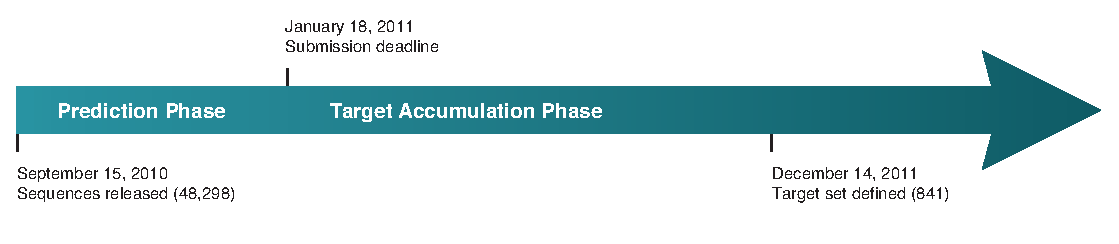
\includegraphics[width=\textwidth]{Figures/intro/NM_1A}
                \label{fig:cafa1}
        \end{subfigure}%

	\begin{subfigure}[b]{0.55\textwidth}
                \centering
                \caption{Target counts}                
                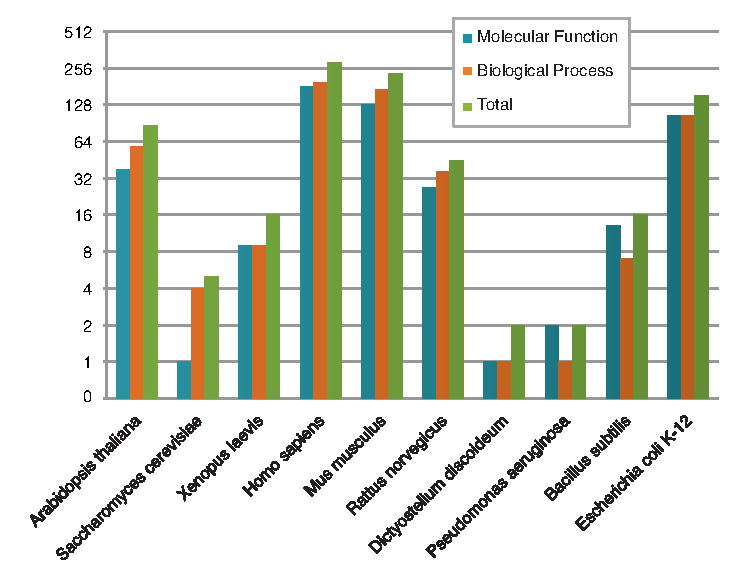
\includegraphics[width=\textwidth]{Figures/intro/NM_1B}
                \label{fig:cafa2}
        \end{subfigure}
	\quad
	\begin{subfigure}[b]{0.30\textwidth}
                \centering
                \caption{Functional terms}                
                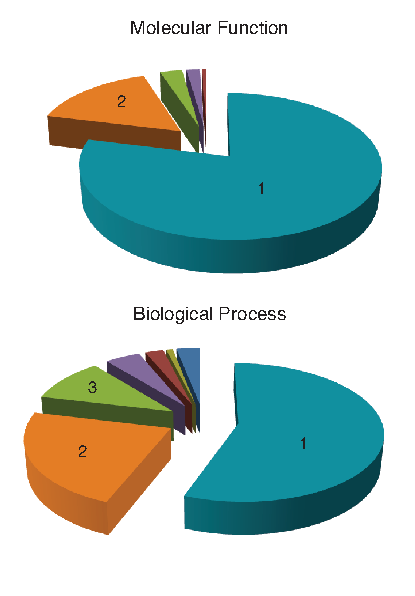
\includegraphics[width=\textwidth]{Figures/intro/NM_1C}
                \label{fig:cafa3}
        \end{subfigure}%

\end{centering}
\caption[CAFA Experiment and data]{\Cref{fig:cafa1}: Timeline for the CAFA experiment. \Cref{fig:cafa2}: Number of target sequences per organism. The graph shows the number of target sequences for each of the ontologies (Molecular Function and Biological Process) as well as the total number of targets, obtained as a union between sequences in the two ontologies. Of 866 proteins, 531 had Molecular Function annotations and 587 had Biological Process annotations. \Cref{fig:cafa3}: Distribution of target sequences in each ontology according to the number of leaf terms available for each protein sequence. For example, in the Molecular Function category, $79\%$ of proteins had one leaf term, $16\%$ had two leaf terms, and so on. A term is considered a leaf term for a particular target if no other GO term associated with that sequence is its descendant.}
\label{fig:SCOP_ROC}
\end{figure*}





Many of the previously listed state of the art methods participated in the community-wide assessment of function prediction (CAFA) in which I took a prominent role \citep{Radivojac2013}. The CAFA experiment was conducted by first creating a data set of $48,298$ proteins that lacked experimentally verified GO annotations in Swiss-Prot.  Participating groups were then asked to submit annotations for this set of proteins before a predetermined deadline.  During the annotation accumulation phase experimental annotations were allowed to accumulated for approximately a year.  This resulted in an evaluation data set of $866$ target sequences, 531 with Molecular Function annotations, and 587 with Biological Process annotations.  Reinforcing the need for advanced methods for function prediction, we consistently found that state of the art methods outperformed inferring function using sequence similarity (in this case BLAST).  Furthermore, BLAST barely outperformed simply using the background distribution of functions as a predictor (Na\"ive).  The BLAST and Na\"ive models are described in \Cref{sec:blast} and \Cref{sec:naive} respectively.

%\begin{figure*}[t!]
%\begin{centering}
%	\begin{subfigure}[b]{0.45\textwidth}
%                \centering
%                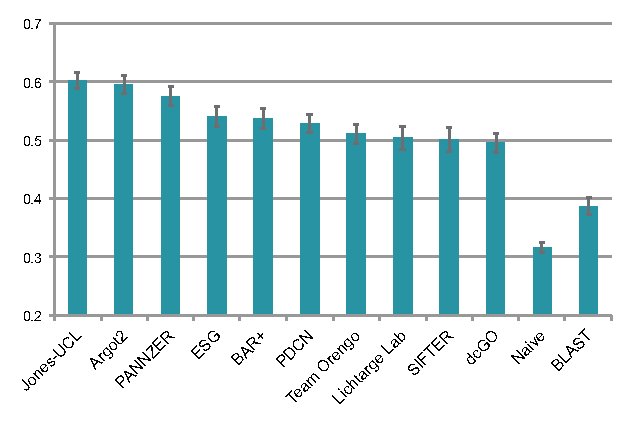
\includegraphics[width=\textwidth]{Figures/intro/dino_mfo}
%                \caption{Molecular Function}
%                \label{fig:dino_mfo}
%        \end{subfigure}%
%        \quad
%        \quad
%	\begin{subfigure}[b]{0.45\textwidth}
%                \centering
%                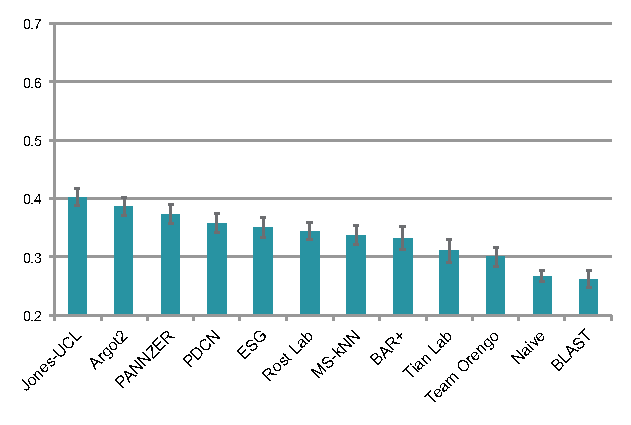
\includegraphics[width=\textwidth]{Figures/intro/dino_bpo}
%                \caption{Biological Process}
%                \label{fig:dino_bpo}
%        \end{subfigure}
%
%\end{centering}
%\caption[Maximum F-measure of the top teams participating in CAFA]{The maximum F-measure for the top-performing methods for Molecular Function ontology (\Cref{fig:dino_mfo}) and Biological Process ontology (\Cref{fig:dino_mfo}). F-max values were calculated as described by \Cref{eq:fmax}. All panels show the top ten participating methods in each category as well as the BLAST (\Cref{sec:blast}) and Naive (\Cref{sec:naive}) baseline methods. Note that 33 models outperformed BLAST in the Molecular Function category, whereas 26 models outperformed BLAST in the Biological Process category (cutoff scores below which methods were excluded from the panels were 0.468 and 0.300 for the Molecular Function and Biological Process categories, respectively). In the Molecular Function category, proteins with ``protein binding" as their only leaf term were excluded from the analysis because the protein binding term was not considered informative. Confidence intervals ($95\%$) were determined using bootstrapping with $n = 10,000$ iterations on the set of target sequences. For cases in which a principal investigator participated in multiple teams, only the results of the best-scoring method are presented.}
%\label{fig:cafadino}
%\end{figure*}



\section{Analysis of function in evolutionary context}

The previous chapters focused largely on the inference of function.  While these endeavors are important in their own right, it is desirable that the data produced by these efforts will at some point; perhaps this point has already arrived, serve as more than an encyclopedic cataloging of the known gene/protein universe. In \Cref{ch:oc} we use several different types of data, including GO annotations, to compare the functional similarity of orthologous and paralogous sequences \citep{Nehrt2011}.  While the results of our findings have implications for the inference of function prediction, especially when phylogenetic data is used \citep{Eisen1998,vskunca2012phyletic}; it also represents a transition from utilizing GO annotations simply to inform a user about a gene, to using both curated and predicted functional annotations to generate and test theories about biology and evolution.


\section{Conclusion}

With the growing gap between known sequences and experimentally annotated proteins, it is clear that functional annotation of all proteins can only be accomplished by combining experimental and computational methods. Targeted wet lab experiments have been predominantly focused on model organisms with an expectation that results will provide a detailed understanding of these organisms and that the gap between species can be accurately filled by computational methods. Indeed, model organisms provide a large fraction of the genes with experimentally verified functional annotations. In Swiss-Prot v15.15, we found that approximately $90\%$ of annotated proteins in molecular function and biological process belong to $9$ model organisms only (\emph{H. sapiens}, \emph{S. cerevisiae}, \emph{M. musculus}, \emph{R. norvegicus}, \emph{A. thaliana}, \emph{D. melanogaster}, \emph{S. pombe}, \emph{E. coli K-12}, and \emph{C. elegans}). However, nearly $60\%$ of the proteins from these model organisms still do not have any experimentally determined molecular function or biological process terms. Thus, the development and assessment of computational methods is critical for not only filling the gap between model and non-model organisms, but also for completing the annotation of model organisms and driving experimental analyses.

A frequent interpretation of the sequence-structure-function paradigm is that a protein must adopt a single structure (minimum energy state, kinetically reachable) in order to be functional, with such conformation usually called the native state. However, such an understanding has been challenged from both structural and functional perspectives. Many proteins have been characterized as intrinsically disordered. In such proteins, no single structure is seen as being dominant (i.e. high probability conformation with deep energy minimum) and a presence of conformational ensembles (i.e. macro states \citep{Dill1999}) is probably even required for function \citep{Dunker2002,Dyson2005a,Radivojac2007}. At the same time, it is now recognized that multifunctional proteins are also common \citep{Jeffery2009}. We find that at least $34\%$ of functionally characterized proteins (by experimental studies) are already assigned more than one distinct molecular function term and that at least $56\%$ of proteins participate in more than one distinct biological process. We believe that the ability of a protein to be multifunctional in terms of its biochemical function needs to be achieved by developing new structural conformations and physicochemical interfaces (including the addition of new domains), whereas its involvement in multiple biological processes does not. This is because an organism need only utilize the given protein in a different context, excluding the necessity to change the actual mechanism through which the protein functions.

We also analyzed the quality of molecular function and biological process term transfer by simple sequence similarity and found that inference by similarity shows flat accuracy in the entire range from $30-100\%$ of pairwise sequence identity (unless within the same organism). This leads to the conclusion that more sophisticated computational methods are necessary. To date, much attention has specifically been paid to the quality of function transfer for enzymes \citep{Addou2009,Rost2003}. Here, we extended such analyses to non-enzymatic proteins and observed that transfer of function to non-enzymatic proteins is less accurate than that achieved for proteins annotated with any function from the catalytic activity portion of the ontology. While the underlying reasons may simply lie in the sparseness of these parts of the ontology, annotating a protein with functions without knowledge of the associated mechanics (information that is often known for enzymes) can result in less accurate assignment of proteins with such terms. This may also be true for other classes of terms in the ontology. For example, terms which group together proteins that carry out similar tasks in the cell, but do so through different molecular mechanisms, will be less likely to be defined in terms of sequence similarity among member proteins. Conversely, terms which define a function carried out by a specific mechanism (e.g. zinc finger binding) will be more likely to be inferred by sequence similarity.

